% Se necesita un motor de LaTeX moderno como LuaLaTeX para compilar el documento
% debido al uso de fontspec y polyglossia
% Puede requerir tener el paquete lmodern instalado
% Se necesita ejecutar el compilador de LaTeX con -shell-escape
% Se necesita crear una carpeta llamada "tikz" en el directorio de compilación

% Declarar documento como tipo "article" a letra 12 puntos y tamaño de papel A4
\documentclass[12pt, a4paper]{article}

% Para poder especificar partes del documento en orientación apaisada
\usepackage{pdflscape}

% Ampliar la superficie de papel usada por el documento
\usepackage[a4paper, total={6.5in, 9.5in}]{geometry}

% Configurar el idioma del documento a español
\usepackage{polyglossia}
\setdefaultlanguage{spanish}

% Generar marcadores de PDF a partir de los capítulos y secciones
\usepackage[bookmarks]{hyperref}

% Paquete para configuración avanzada de fuentes y uso de fuentes en
% formatos TTF y OTF
% Para que funcione es necesario usar un motor de LaTeX que lo
% soporte como LuaLaTeX
% https://en.wikibooks.org/wiki/LaTeX/Fonts#Using_TTF_and_OTF_fonts
\usepackage{fontspec}

% Paquete con herramientas para manejar colores en el documento
\usepackage[dvipsnames]{xcolor}

% Definiciones de color personalizadas
% Comentarios en bloques de código (verde)
\definecolor{code_comment}{rgb}{0, 0.5, 0}

% Paquete de herramientas matemáticas mejoradas
% https://en.wikibooks.org/wiki/LaTeX/Mathematics
% https://www.overleaf.com/learn/latex/Mathematical_expressions
% https://en.wikibooks.org/wiki/LaTeX/Advanced_Mathematics
\usepackage{mathtools}

% Símbolos matemáticos de la American Mathematical Society
% Entre estos símbolos se encuentran los que se usan para identificar
% conjuntos numéricos notables
% como el conjunto de los números enteros, números reales...
\usepackage{amssymb}

% Permite el posicionamiento preciso de figuras en la misma línea en
% la que se declaran
% https://www.overleaf.com/learn/latex/Positioning_images_and_tables#The_table_environment
\usepackage{float}

% Paquete que permite la creación de subfiguras dentro de un entorno de figura
% https://www.overleaf.com/learn/latex/Positioning_images_and_tables#Multiple_images_in_one_figure
\usepackage{subcaption}

% Paquete para poder declarar bloques de código con estilos
\usepackage{listings}

% Configuración general para los bloques de código
% https://en.wikibooks.org/wiki/LaTeX/Source_Code_Listings#Settings
\lstset{
    % Estilo del código
    basicstyle=\ttfamily,
    % Estilo de los comentarios
    commentstyle=\color{code_comment},
    % Habilitar numeración de líneas de código
    numbers=left,
    % Estilo de numeración de líneas de código
    numberstyle=\ttfamily,
    breaklines=true
}

% Paquete para poder crear bordes alrededor del espacio que ocupa un entorno
\usepackage{framed}

% Paquete general para gráficos
% https://www.overleaf.com/learn/latex/TikZ_package
\usepackage{tikz}

% Paquete para crear diagramas
% https://www.overleaf.com/learn/latex/Pgfplots_package
\usepackage{pgfplots}

% Configurar versión de compatibilidad de pgfplots
% https://www.overleaf.com/learn/latex/Pgfplots_package#The_document_preamble
\pgfplotsset{compat=1.18}

% Habilitar generación de gráficas como archivos por separado
% Esto hace que el documento se compile más rápido ya que solo vuelve a generar
% las gráficas cuando estas son modificadas
% Para que el documento compile correctamente el motor de compilación se debe
% ejecutar con el argumento -shell-escape y se debe crear una carpeta
% llamada "tikz"
% en el directorio de compilación
\usetikzlibrary{external}
\usepgfplotslibrary{external}
\tikzexternalize[prefix=tikz/]

% Paquete para añadir imágenes
\usepackage{graphicx}
% Especificar directorio de imágenes
\graphicspath{ {./practica_4_memoria_resources/} }

% Paquete para bibliografías
% https://www.overleaf.com/learn/latex/Bibliography_management_with_biblatex
% https://en.wikibooks.org/wiki/LaTeX/Bibliography_Management
% https://en.wikibooks.org/wiki/LaTeX/Bibliography_Management#biblatex
\usepackage{biblatex}

% Añadir el archivo de referencias bibliográficas
% \addbibresource{practica_4_memoria.bib}

% Definir un tipo de encabezado para bibliografías que permite
% generar una sección
% nueva con cada bibliografía que lo usa
\defbibheading{biblatex_encabezado_como_seccion}{
\section{Bibliografía}}

% Para crear tablas en base a archivos CSV
\usepackage[l3]{csvsimple}

\begin{document}
% Portada personalizada
% https://en.wikibooks.org/wiki/LaTeX/Title_Creation#Create_a_custom_title_for_a_report_or_book
\begin{titlepage}
    % Centrar todo el contenido de la portada
    \centering

    % Nombre de la universidad en mayúsculas pequeñas (small caps)
    {\LARGE \textsc{Universidad Rey Juan Carlos} \par}

    % Nombre del grado
    {\Large Grado en Ingeniería de Computadores \par}

    % Curso
    {\large Curso 2024-2025 \par}

    % Espacio vertical
    \vspace{8cm}

    % Nombre de la asignatura
    {\Large \textsc{Fundamentos de diseño de software} \par}

    % Espacio vertical
    \vspace{0.5cm}

    % Número de la práctica
    {\huge Práctica 4: \par}

    % Nombre de la práctica en negrita
    {\Huge \bfseries Backtracking \par}

    % Espacio vertical hasta abajo de la hoja
    \vfill

    % Autores
    {\LARGE Guillermo Baranda Rodríguez \par}
    {\LARGE Daniel Hernández Téllez \par}
    {\LARGE Alonso Martín Arroyo \par}
    {\LARGE Pablo Peral Camúñez \par}
\end{titlepage}

\section{Introducción}

En esta práctica utilizaremos la técnica de backtracking para
resolver obtener el conjunto de caminos (abiertos y cerrados) que
permiten recorrer todo un tablero de ajedrez de dimensiones
arbitrarias pasando una sola vez por cada casilla.

\section{Algoritmo}

\subsection{Una sola solución}

\begin{lstlisting}[language=Java]
boolean buscar(List<Camino> lista, Tablero tablero, Camino camino_temporal, boolean debe_ser_cerrado) throws InterruptedException {
    boolean exito = false;

    /*
    * Conjunto de candidatos: El conjunto de casillas obtenidas a
    * partir de los 8 desplazamientos predefinidos
    */
    for (int candidato = 0; candidato < AlgoritmoUna.candidatos.length && !exito; candidato++) {
        if (Thread.interrupted()) {
            throw new InterruptedException();
        }
        try {
            Casilla siguiente_casilla = tablero.getCasilla(
                    Vec2.add(camino_temporal.getLast().coordenada, candidatos[candidato]));

            /*
            * Función de factibilidad: Comprobar que la casilla
            * exista (excepción TableroCoordenadaFueraDeRango)
            * y que no haya sido recorrida previamente
            */
            if (!siguiente_casilla.recorrida) {
                /*
                * Anotar la solución: Marcar la casilla como
                * recorrida y añadirla al camino recorrido
                */
                siguiente_casilla.recorrida = true;
                camino_temporal.add(siguiente_casilla);

                /*
                * Función de solución: Comprobar que se han
                * recorrido todas las casillas del tablero y,
                * en el caso de que sea necesario, que se
                * pueda ir desde la última casilla del camino
                * a la primera en un solo movimiento
                */
                if ((camino_temporal.size() == tablero.casillas_totales)
                        && (debe_ser_cerrado ? caminoCerrado(camino_temporal, tablero) : true)) {
                    exito = true;
                    lista.add((Camino) camino_temporal.clone());
                } else {
                    /*
                    * Cuando no se ha llegado a la última
                    * casilla, aún no se ha alcanzado una
                    solución por lo que seguimos buscando.
                    */
                    exito = buscar(lista, tablero, camino_temporal, debe_ser_cerrado);
                    if (!exito) {
                        siguiente_casilla.recorrida = false;
                        camino_temporal.removeLast();
                    }
                }
            }
        } catch (TableroCoordenadaFueraDeRango e) {
            // Pasar al siguiente candidato
        }
    }
    if (lista.size() > 1) {
        throw new RuntimeException(
                "ERROR: La lista de caminos generada tiene más de un elemento a pesar de haber sido generada utilizando el algoritmo de una sola solución.");
    }
    return exito;
}
\end{lstlisting}

\subsection{Todas las soluciones}

\begin{lstlisting}[language=Java]
boolean buscar(List<Camino> lista, Tablero tablero, Camino camino_temporal, boolean debe_ser_cerrado) throws InterruptedException {
    /*
    * Conjunto de candidatos: El conjunto de casillas obtenidas
    * a partir de los 8 desplazamientos predefinidos
    */
    for (int candidato = 0; candidato < candidatos.length; candidato++) {
        if (Thread.interrupted()) {
            throw new InterruptedException();
        }
        try {
            Casilla siguiente_casilla = tablero.getCasilla(
                    Vec2.add(camino_temporal.getLast().coordenada, candidatos[candidato]));

            /*
            * Función de factibilidad: Comprobar que la casilla
            * exista (excepción TableroCoordenadaFueraDeRango)
            * y que no haya sido recorrida previamente
            */
            if (!siguiente_casilla.recorrida) {
                /*
                * Anotar la solución: Marcar la casilla como
                * recorrida y añadirla al camino recorrido
                */
                siguiente_casilla.recorrida = true;
                camino_temporal.add(siguiente_casilla);

                /*
                * Función de solución: Comprobar que se han
                * recorrido todas las casillas del tablero
                * y, en el caso de que sea necesario, que
                * se pueda ir desde la última casilla del
                * camino a la primera en un solo movimiento
                */
                if ((camino_temporal.size() == tablero.casillas_totales)
                        && (debe_ser_cerrado ? caminoCerrado(camino_temporal, tablero) : true)) {
                    lista.add((Camino) camino_temporal.clone());
                } else {
                    /*
                    * Cuando no se ha llegado a la última
                    * casilla, aún no se ha alcanzado una
                    * solución por lo que seguimos buscando.
                    */
                    buscar(lista, tablero, camino_temporal, debe_ser_cerrado);
                }
                siguiente_casilla.recorrida = false;
                camino_temporal.removeLast();
            }
        } catch (TableroCoordenadaFueraDeRango e) {
            // Pasar al siguiente candidato
        }
    }
    return lista.size() > 0;
}
\end{lstlisting}

\subsection{Validación de caminos cerrados}

\begin{lstlisting}[language=Java]
boolean caminoCerrado(Camino camino, Tablero tablero) {
    boolean resultado = false;
    for (int candidato = 0; candidato < candidatos.length && !resultado; candidato++) {
        try {
            Casilla siguiente_casilla = tablero.getCasilla(
                    Vec2.add(camino.getLast().coordenada, candidatos[candidato]));
            if (siguiente_casilla == camino.getFirst()) {
                resultado = true;
            }
        } catch (TableroCoordenadaFueraDeRango e) {
        }
    }
    return resultado;
}
\end{lstlisting}

\section{Tablas de prueba}

\textit{
    Nota: Nuestro sistema de pruebas posee de un mecanismo de
    paro automático de las pruebas pasado un tiempo límite
    preestablecido. Aquellas pruebas que hayan sido interrumpidas
    por superar el tiempo límite establecido tendrán como valor de tiempo de
    ejecución el tiempo límite establecido precedido de un símbolo de
    mayor que ($>$) para señalar que el tiempo de ejecución real de
    la prueba es superior a dicho valor.
}

\begin{figure}[H]
    \begin{center}
        \label{tab:basicos}
        \caption{Casos de prueba básicos}

        \begin{tabular}{|c|c|c|c|c|}
            \hline
            % Cabecera de la tabla (todo en negrita)
            \textbf{Tamaño} & \textbf{Abierto} & \textbf{Cerrado} &
            \textbf{Tiempo abierto (ms)} & \textbf{Tiempo cerrado (ms)}
            \csvreader[head to column names]
            {resultados_pruebas/Tabla 1 - Soluciones simples.csv}
            % Asignaciones adicionales de nombre de columna
            {
                {TIEMPO ABIERTO (ms)}=\TIEMPOABIERTO,
                {TIEMPO CERRADO (ms)}=\TIEMPOCERRADO
            }
            {
                \\ \hline \TAMAÑO & \ABIERTO & \CERRADO & \TIEMPOABIERTO
                & \TIEMPOCERRADO
            }
            \\ \hline
        \end{tabular}
    \end{center}
\end{figure}

\begin{figure}[H]
    \begin{center}
        \label{tab:complejos}
        \caption{Casos de prueba complejos}

        \begin{tabular}{|c|c|c|c|c|}
            \hline
            % Cabecera de la tabla (todo en negrita)
            \textbf{Tamaño} & \textbf{Abierto} & \textbf{Cerrado} &
            \textbf{Tiempo abierto (ms)} & \textbf{Tiempo cerrado (ms)}
            \csvreader[head to column names]
            {resultados_pruebas/Tabla 2 - Soluciones complejas.csv}
            % Asignaciones adicionales de nombre de columna
            {
                {TIEMPO ABIERTO (ms)}=\TIEMPOABIERTO,
                {TIEMPO CERRADO (ms)}=\TIEMPOCERRADO
            }
            {
                \\ \hline \TAMAÑO & \ABIERTO & \CERRADO & \TIEMPOABIERTO
                & \TIEMPOCERRADO
            }
            \\ \hline
        \end{tabular}
    \end{center}
\end{figure}

\begin{figure}[H]
    \begin{center}
        \label{tab:todas_soluciones}
        \caption{Casos de prueba de la variante de todas las soluciones}

        \begin{tabular}{|c|c|c|c|c|}
            \hline
            % Cabecera de la tabla (todo en negrita)
            \textbf{Tamaño} & \textbf{Abierto} & \textbf{Cerrado} &
            \textbf{Tiempo abierto (ms)} & \textbf{Tiempo cerrado (ms)}
            \csvreader[head to column names]
            {resultados_pruebas/Tabla 3 - Todas las soluciones.csv}
            % Asignaciones adicionales de nombre de columna
            {
                {TIEMPO ABIERTO (ms)}=\TIEMPOABIERTO,
                {TIEMPO CERRADO (ms)}=\TIEMPOCERRADO
            }
            {
                \\ \hline \TAMAÑO & \ABIERTO & \CERRADO & \TIEMPOABIERTO
                & \TIEMPOCERRADO
            }
            \\ \hline
        \end{tabular}
    \end{center}
\end{figure}

\section{Preguntas}

\begin{itemize}
    \item \textbf{¿Cuántos niveles tendrá el árbol de exploración? ¿Y
        en el caso del camino cerrado?:} Es necesario que el árbol de
        exploración tenga igual número de casillas del tablero, ya
        que cada nivel sería una casilla que tiene que recorrer el
        caballo, y evidentemente no se pueden repetir.
        En el caso de que sea cerrado, implicaría que desde la
        casilla final se puede retroceder a la inicial. Esto
        significa que los niveles en sí del árbol no cambiarían, ya
        que no generaría ningún nivel nuevo.
    \item \textbf{¿Cuántos candidatos tendrá el árbol de exploración
        en cada nivel?:} Los candidatos corresponden al número de
        movimientos que puede hacer el caballo en la casilla en la
        que esté, siempre y cuando se cumpla que la casilla esté
        dentro del tablero y no haya sido visitada aún.
        En teoría, el número máximo de candidatos es 8, que es el
        número máximo de movimientos diferentes posibles del caballo, pero
        el número exacto depende de la posición en la que estemos. Si el caballo
        está en una esquina, el rango de movimientos se reduce un
        cuarto, y a medida que vamos avanzando, va disminuyendo el
        número de candidatos viables ya que se van recorriendo casillas.
        Así que el máximo teórico son 8, y el número real depende de
        la posición de cada casilla en el tablero y de las casillas
        recorridas hasta el momento.
    \item \textbf{¿Cómo influyen los tiempos en caso de modificar la
        casilla inicial o el orden de las casillas candidatas?:}
        Con respecto a la casilla inicial, cambiarla a la
        casilla central del tablero podría reducir el tiempo necesario
        para encontrar un primer camino debido a que el número de candidatos
        sería el máximo posible para el tablero.

        Con respecto al orden de las casillas candidatas, debido a
        los pares de casillas próximos entre sí, podría resultar más
        óptimo recorrer la lista de casillas candidatas alternando
        entre las distintas esquinas en vez de en sentido
        anti-horario. Por ejemplo:

        \begin{center}
            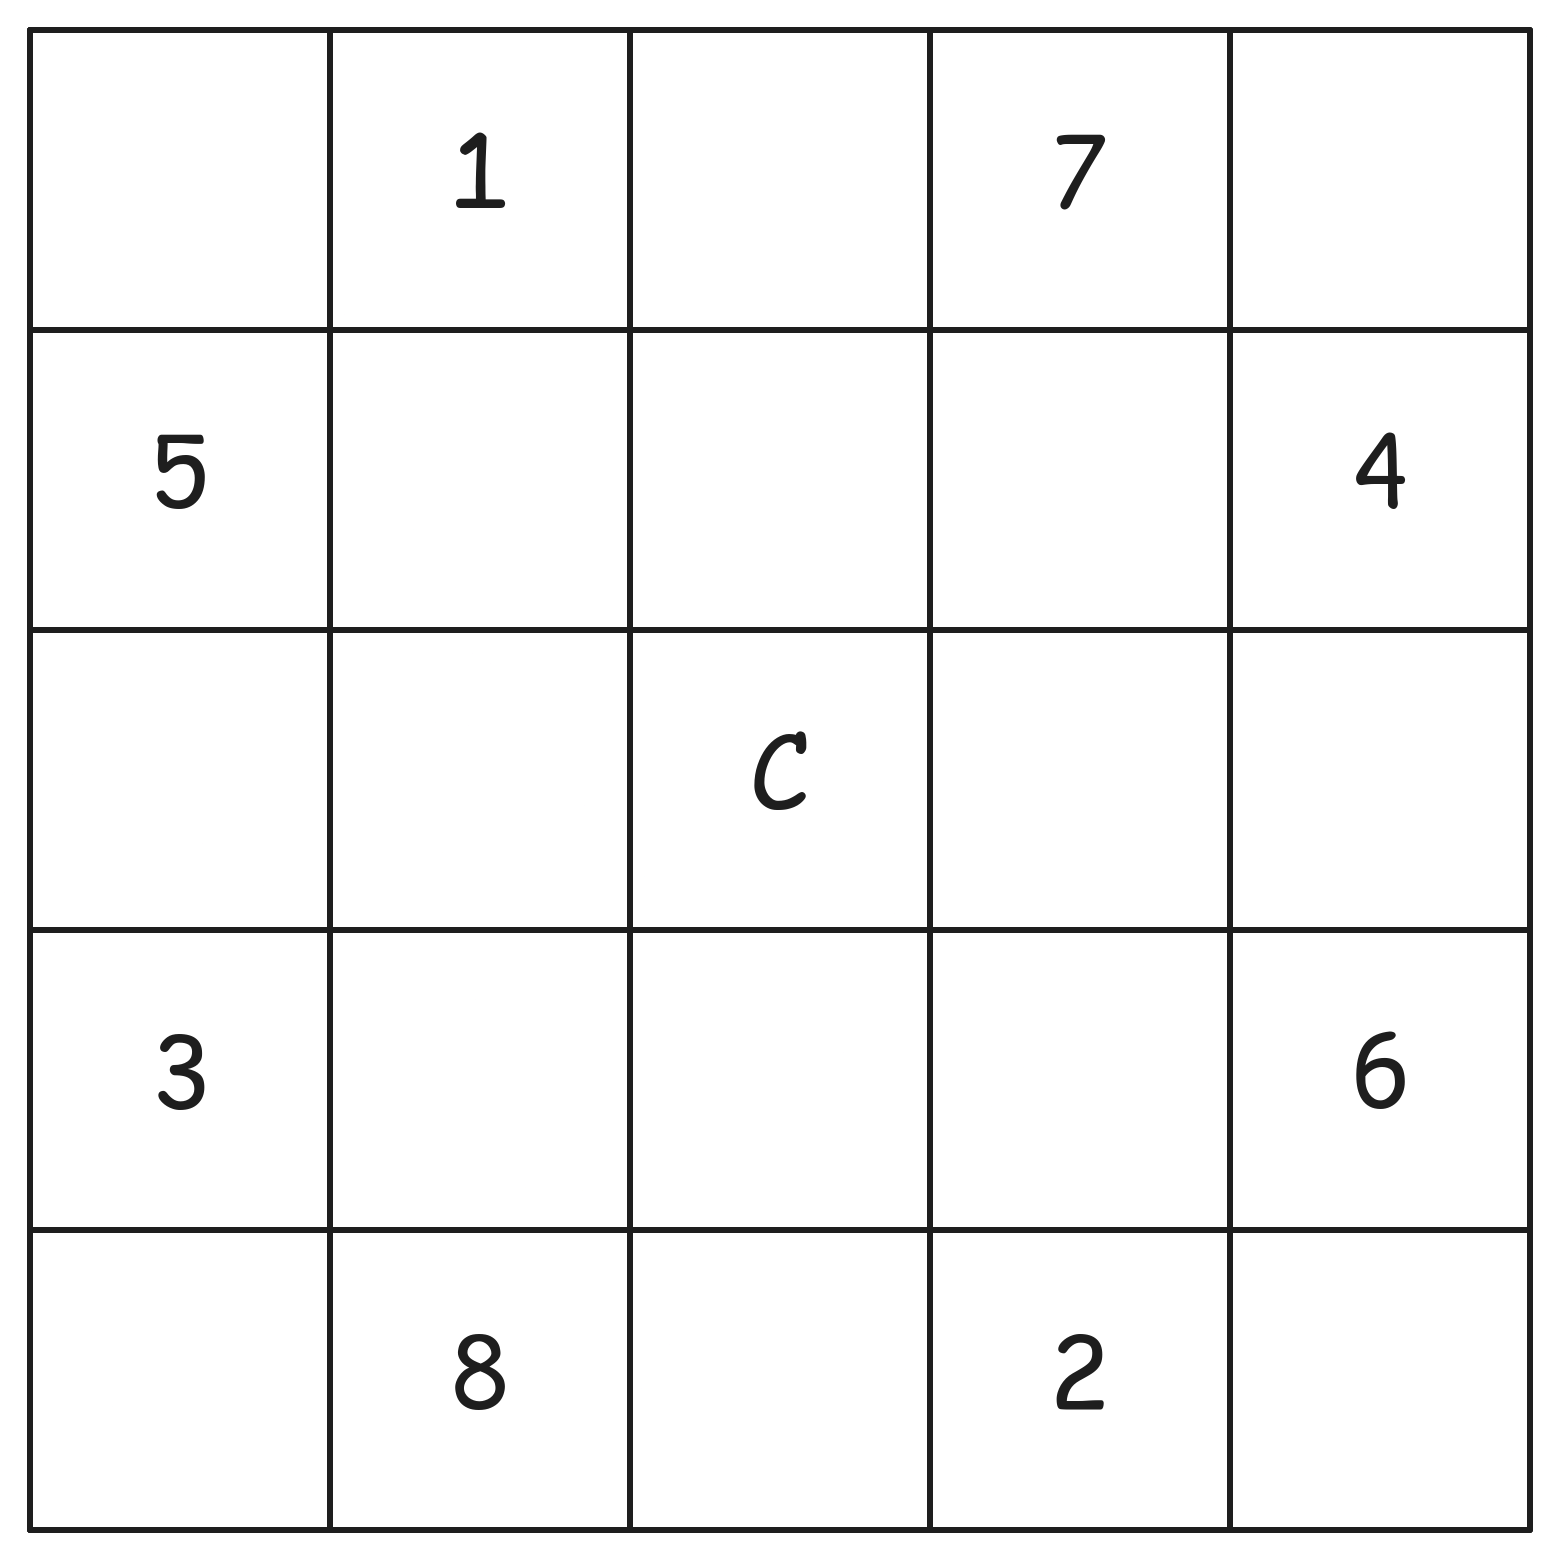
\includegraphics[width=0.25\textwidth]{nuevo_orden_casillas_candidatas.excalidraw.png}
        \end{center}
\end{itemize}

\section{Conclusiones}

En esta práctica hemos aprendido a utilizar algoritmos de vuelta
atrás y evaluación de combinaciones utilizando árboles de navegación.
Uno de los aspectos más complejos de la práctica ha sido la
implementación del mecanismo de parada automática de las pruebas
debido a la necesidad de usar hilos de ejecución adicionales para
controlar la ejecución del algoritmo.

\begin{landscape}
    \section{Resultados de las pruebas simples y complejas}

    \lstinputlisting[numbers=none,basicstyle=\ttfamily\tiny]{resultados_pruebas/Caminos.txt}
\end{landscape}

\end{document}
